\documentclass{article} % say
\usepackage{graphics}
\usepackage{transparent}
\usepackage[dvipsnames]{xcolor}
\usepackage{tikz}
\usetikzlibrary{decorations.pathreplacing,angles,quotes}
\pgfrealjobname{figure}

\begin{document}
\begin{figure}
\beginpgfgraphicnamed{fig1}

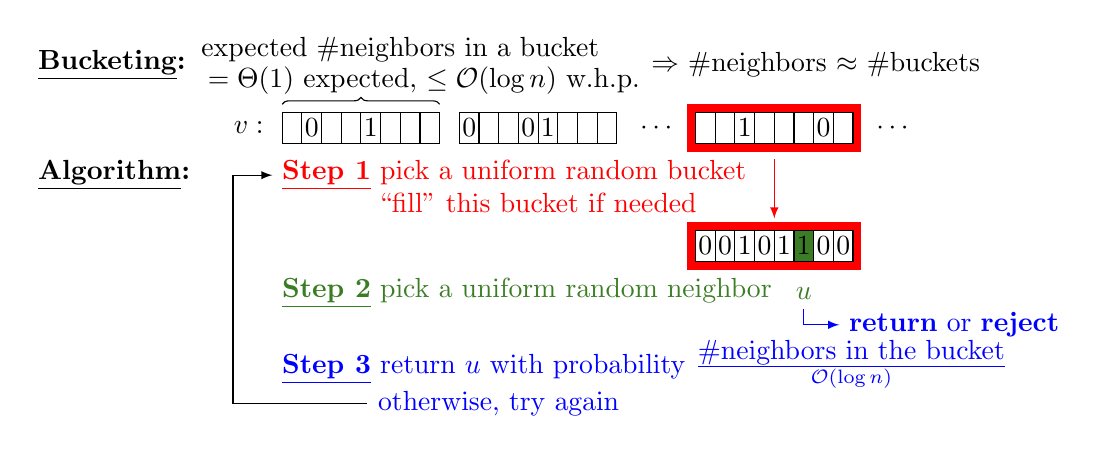
\begin{tikzpicture}
\begin{scope}[>=latex]
\filldraw[fill=red,draw=red] (6.375,0) + (-1.1,-.3) rectangle ++(1.1,.3);
\filldraw[fill=red,draw=red] (6.375,-1.5) + (-1.1,-.3) rectangle ++(1.1,.3);
\foreach \x in {1,2,...,8}
{
\filldraw[fill=white] (\x/4,0) + (-.125,-.2) rectangle ++(.125,.2);
\filldraw[fill=white] (\x/4+2.25,0) + (-.125,-.2) rectangle ++(.125,.2);
\filldraw[fill=white] (\x/4+5.25,0) + (-.125,-.2) rectangle ++(.125,.2);
\filldraw[fill=white] (\x/4+5.25,-1.5) + (-.125,-.2) rectangle ++(.125,.2);
}
\filldraw[fill=OliveGreen] (6.75,-1.5) + (-.125,-.2) rectangle ++(.125,.2);


\draw[decoration={brace},decorate] (.125, .3) -- node[above] {} (2.125,.3);
\draw (1.125+.5,1) node{expected \#neighbors in a bucket};
\draw (1.125+.8,.6) node{$=\Theta(1)$ expected, $\leq \mathcal{O}(\log n)$ w.h.p.};
%\draw[decoration={brace},decorate] (4.75, 1.2) -- node {} (4.75,.4);
\draw (6.9,0.8) node{$\Rightarrow$ \#neighbors $\approx$ \#buckets};

\draw (-0.3,0) node{$v:$};
\draw (4.875,0) node{$\cdots$};
\draw (7.875,0) node{$\cdots$};
\draw (.5,0) node{0};
\draw (1.25,0) node{1};
\draw (2.5,0) node{0};
\draw (3.25,0) node{0};
\draw (3.5,0) node{1};
\draw (6,0) node{1};
\draw (7,0) node{0};

\draw (5.5,-1.5) node{0};
\draw (5.75,-1.5) node{0};
\draw (6,-1.5) node{1};
\draw (6.25,-1.5) node{0};
\draw (6.5,-1.5) node{1};
\draw (6.75,-1.5) node{1};
\draw (7,-1.5) node{0};
\draw (7.25,-1.5) node{0};
\draw (6.75,-2.1) node{\color{OliveGreen}$u$};

\draw[->,draw=red] (6.375,-0.4) -- (6.375,-1.15);
\draw[->,draw=blue] (6.75,-2.3) -- (6.75,-2.5) -- (7.2,-2.5);

\draw (-3.1, -.6) node[right=0mm] {\textbf{\underline{Algorithm}:}};
\draw (-3.1, 0.8) node[right=0mm] {\textbf{\underline{Bucketing}:}};

\draw (0, -.6) node[right=0mm] {\color{red}\underline{\textbf{Step 1}} pick a uniform random bucket};
\draw (1.22, -0.95) node[right=0mm] {\color{red}``fill'' this bucket if needed};

\draw (0, -2.1) node[right=0mm] {\color{OliveGreen}\underline{\textbf{Step 2}} pick a uniform random neighbor};

\draw (0, -3) node[right=0mm] {\color{blue}\underline{\textbf{Step 3}} return $u$ with probability $\frac{\textrm{\#neighbors in the bucket}}{\mathcal{O}(\log n)}$};
\draw (1.22, -3.5) node[right=0mm] {\color{blue}otherwise, try again};
\draw (7.2, -2.5) node[right=0mm] {\color{blue} \textbf{return} or \textbf{reject}};

\draw[->] (1.2,-3.5) -- (-0.5,-3.5) -- (-0.5,-0.6) -- (0, -0.6);
\end{scope}
\end{tikzpicture}
\endpgfgraphicnamed
\end{figure}

\begin{figure}
\beginpgfgraphicnamed{fig2}
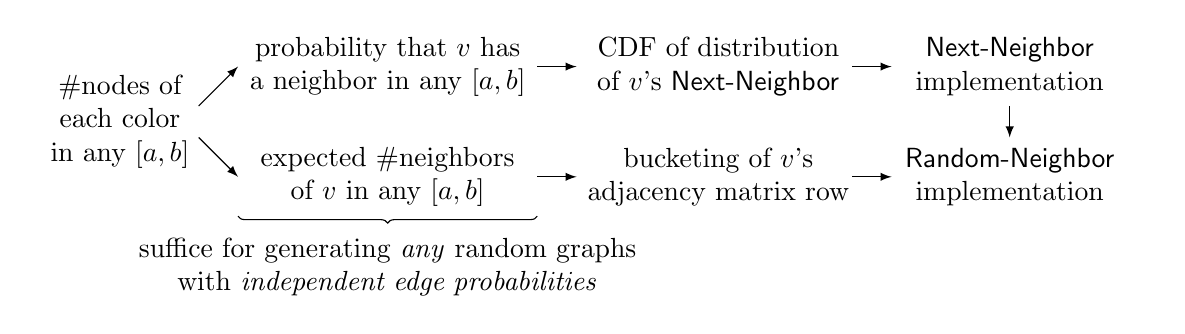
\begin{tikzpicture}

\begin{scope}[>=latex]
\draw[text width=60,text centered] (0,0) node {\#nodes of each color in any $[a,b]$};
\draw[text width=100,text centered] (3.4,.7) node {probability that $v$ has a neighbor in any $[a,b]$};
\draw[text width=100,text centered] (7.6,.7) node {CDF of distribution of $v$'s \textsf{Next-Neighbor}};
\draw[text width=100,text centered] (11.3,.7) node {\textsf{Next-Neighbor} implementation};
\draw[text width=100,text centered] (3.4,-.7) node {expected \#neighbors of $v$ in any $[a,b]$};
\draw[text width=100,text centered] (7.6,-.7) node {bucketing of $v$'s adjacency matrix row};
\draw[text width=100,text centered] (11.3,-.7) node {\textsf{Random-Neighbor} implementation};
\draw[->] (1,.2) -- (1.5,.7);
\draw[->] (1,-.2) -- (1.5,-.7);
\draw[->] (5.3,.7) -- (5.8,.7);
\draw[->] (5.3,-.7) -- (5.8,-.7);
\draw[->] (9.3,.7) -- (9.8,.7);
\draw[->] (9.3,-.7) -- (9.8,-.7);
\draw[->] (11.3,.2) -- (11.3,-.2);
\draw[decoration={brace},decorate] (5.3, -1.2) -- node[below] {} (1.5,-1.2);
\draw[text width=200,text centered] (3.4,-1.85) node {suffice for generating \emph{any} random graphs with \emph{independent edge probabilities}};

\end{scope}
\end{tikzpicture}
\endpgfgraphicnamed
\end{figure}

\begin{figure}
\beginpgfgraphicnamed{fig3}

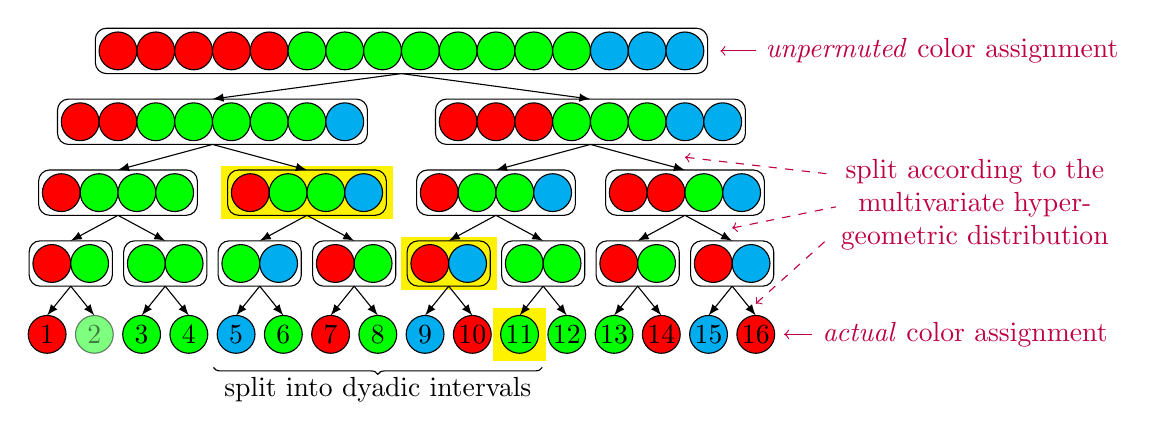
\begin{tikzpicture}
\def\s{0.6}
\def\r{0.4*\s}
\begin{scope}[>=latex]

\draw[fill=yellow,draw=yellow] (10*\s,0) + (-0.55*\s,-0.55*\s) rectangle ++(0.55*\s,0.55*\s);
\draw[fill=yellow,draw=yellow] (8.5*\s,1.5*\s) + (-\s,-0.55*\s) rectangle ++(\s,0.55*\s);
\draw[fill=yellow,draw=yellow] (5.5*\s,3*\s) + (-1.8*\s,-0.55*\s) rectangle ++(1.8*\s,0.55*\s);


\foreach \x in {0,1,...,7}{
\draw[rounded corners] (.5*\s+2*\x*\s,1.5*\s) + (-2.2*\r,-1.2*\r) rectangle ++(2.2*\r,1.2*\r);
\draw[->] (.5*\s+2*\x*\s,1.5*\s-1.2*\r) -- (2*\x*\s,\r);
\draw[->] (.5*\s+2*\x*\s,1.5*\s-1.2*\r) -- (2*\x*\s+\s,\r);
}
\foreach \x in {0,1,...,3}{
\draw[rounded corners] (1.5*\s+4*\x*\s,3*\s) + (-4.2*\r,-1.2*\r) rectangle ++(4.2*\r,1.2*\r);
\draw[->] (1.5*\s+4*\x*\s,3*\s-1.2*\r) -- (4*\x*\s+0.5*\s,1.5*\s+1.2*\r);
\draw[->] (1.5*\s+4*\x*\s,3*\s-1.2*\r) -- (4*\x*\s+2.5*\s,1.5*\s+1.2*\r);
}
\foreach \x in {0,1}{
\draw[rounded corners] (3.5*\s+8*\x*\s,4.5*\s) + (-8.2*\r,-1.2*\r) rectangle ++(8.2*\r,1.2*\r);
\draw[->] (3.5*\s+8*\x*\s,4.5*\s-1.2*\r) -- (8*\x*\s+1.5*\s,3*\s+1.2*\r);
\draw[->] (3.5*\s+8*\x*\s,4.5*\s-1.2*\r) -- (8*\x*\s+5.5*\s,3*\s+1.2*\r);
}
\foreach \x in {0}{
\draw[rounded corners] (7.5*\s+16*\x*\s,6*\s) + (-16.2*\r,-1.2*\r) rectangle ++(16.2*\r,1.2*\r);
\draw[->] (7.5*\s+16*\x*\s,6*\s-1.2*\r) -- (16*\x*\s+3.5*\s,4.5*\s+1.2*\r);
\draw[->] (7.5*\s+16*\x*\s,6*\s-1.2*\r) -- (16*\x*\s+11.5*\s,4.5*\s+1.2*\r);
}

\renewcommand\transparent[1]{}%
\transparent{0.5}\draw[fill=red] (0,0) circle (\r) node{1};
\draw[fill=green, opacity=0.5] (\s,0) circle (\r) node{2};
\draw[fill=green] (2*\s,0) circle (\r) node{3};
\draw[fill=green] (3*\s,0) circle (\r) node{4};
\draw[fill=cyan] (4*\s,0) circle (\r) node{5};
\draw[fill=green] (5*\s,0) circle (\r) node{6};
\draw[fill=red] (6*\s,0) circle (\r) node{7};
\draw[fill=green] (7*\s,0) circle (\r) node{8};
\draw[fill=cyan] (8*\s,0) circle (\r) node{9};
\draw[fill=red] (9*\s,0) circle (\r) node{10};
\draw[fill=green] (10*\s,0) circle (\r) node{11};
\draw[fill=green] (11*\s,0) circle (\r) node{12};
\draw[fill=green] (12*\s,0) circle (\r) node{13};
\draw[fill=red] (13*\s,0) circle (\r) node{14};
\draw[fill=cyan] (14*\s,0) circle (\r) node{15};
\draw[fill=red] (15*\s,0) circle (\r) node{16};

\draw[fill=red] (0.5*\s-\r,1.5*\s) circle (\r);
\draw[fill=green] (0.5*\s+\r,1.5*\s) circle (\r);
\draw[fill=green] (2.5*\s-\r,1.5*\s) circle (\r);
\draw[fill=green] (2.5*\s+\r,1.5*\s) circle (\r);
\draw[fill=green] (4.5*\s-\r,1.5*\s) circle (\r);
\draw[fill=cyan] (4.5*\s+\r,1.5*\s) circle (\r);
\draw[fill=red] (6.5*\s-\r,1.5*\s) circle (\r);
\draw[fill=green] (6.5*\s+\r,1.5*\s) circle (\r);
\draw[fill=red] (8.5*\s-\r,1.5*\s) circle (\r);
\draw[fill=cyan] (8.5*\s+\r,1.5*\s) circle (\r);
\draw[fill=green] (10.5*\s-\r,1.5*\s) circle (\r);
\draw[fill=green] (10.5*\s+\r,1.5*\s) circle (\r);
\draw[fill=red] (12.5*\s-\r,1.5*\s) circle (\r);
\draw[fill=green] (12.5*\s+\r,1.5*\s) circle (\r);
\draw[fill=red] (14.5*\s-\r,1.5*\s) circle (\r);
\draw[fill=cyan] (14.5*\s+\r,1.5*\s) circle (\r);

\draw[fill=red] (1.5*\s-3*\r,3*\s) circle (\r);
\draw[fill=green] (1.5*\s-\r,3*\s) circle (\r);
\draw[fill=green] (1.5*\s+\r,3*\s) circle (\r);
\draw[fill=green] (1.5*\s+3*\r,3*\s) circle (\r);
\draw[fill=red] (5.5*\s-3*\r,3*\s) circle (\r);
\draw[fill=green] (5.5*\s-\r,3*\s) circle (\r);
\draw[fill=green] (5.5*\s+\r,3*\s) circle (\r);
\draw[fill=cyan] (5.5*\s+3*\r,3*\s) circle (\r);
\draw[fill=red] (9.5*\s-3*\r,3*\s) circle (\r);
\draw[fill=green] (9.5*\s-\r,3*\s) circle (\r);
\draw[fill=green] (9.5*\s+\r,3*\s) circle (\r);
\draw[fill=cyan] (9.5*\s+3*\r,3*\s) circle (\r);
\draw[fill=red] (13.5*\s-3*\r,3*\s) circle (\r);
\draw[fill=red] (13.5*\s-\r,3*\s) circle (\r);
\draw[fill=green] (13.5*\s+\r,3*\s) circle (\r);
\draw[fill=cyan] (13.5*\s+3*\r,3*\s) circle (\r);

\draw[fill=red] (3.5*\s-7*\r,4.5*\s) circle (\r);
\draw[fill=red] (3.5*\s-5*\r,4.5*\s) circle (\r);
\draw[fill=green] (3.5*\s-3*\r,4.5*\s) circle (\r);
\draw[fill=green] (3.5*\s-\r,4.5*\s) circle (\r);
\draw[fill=green] (3.5*\s+\r,4.5*\s) circle (\r);
\draw[fill=green] (3.5*\s+3*\r,4.5*\s) circle (\r);
\draw[fill=green] (3.5*\s+5*\r,4.5*\s) circle (\r);
\draw[fill=cyan] (3.5*\s+7*\r,4.5*\s) circle (\r);
\draw[fill=red] (11.5*\s-7*\r,4.5*\s) circle (\r);
\draw[fill=red] (11.5*\s-5*\r,4.5*\s) circle (\r);
\draw[fill=red] (11.5*\s-3*\r,4.5*\s) circle (\r);
\draw[fill=green] (11.5*\s-\r,4.5*\s) circle (\r);
\draw[fill=green] (11.5*\s+\r,4.5*\s) circle (\r);
\draw[fill=green] (11.5*\s+3*\r,4.5*\s) circle (\r);
\draw[fill=cyan] (11.5*\s+5*\r,4.5*\s) circle (\r);
\draw[fill=cyan] (11.5*\s+7*\r,4.5*\s) circle (\r);

\draw[fill=red] (7.5*\s-15*\r,6*\s) circle (\r);
\draw[fill=red] (7.5*\s-13*\r,6*\s) circle (\r);
\draw[fill=red] (7.5*\s-11*\r,6*\s) circle (\r);
\draw[fill=red] (7.5*\s-9*\r,6*\s) circle (\r);
\draw[fill=red] (7.5*\s-7*\r,6*\s) circle (\r);
\draw[fill=green] (7.5*\s-5*\r,6*\s) circle (\r);
\draw[fill=green] (7.5*\s-3*\r,6*\s) circle (\r);
\draw[fill=green] (7.5*\s-\r,6*\s) circle (\r);
\draw[fill=green] (7.5*\s+\r,6*\s) circle (\r);
\draw[fill=green] (7.5*\s+3*\r,6*\s) circle (\r);
\draw[fill=green] (7.5*\s+5*\r,6*\s) circle (\r);
\draw[fill=green] (7.5*\s+7*\r,6*\s) circle (\r);
\draw[fill=green] (7.5*\s+9*\r,6*\s) circle (\r);
\draw[fill=cyan] (7.5*\s+11*\r,6*\s) circle (\r);
\draw[fill=cyan] (7.5*\s+13*\r,6*\s) circle (\r);
\draw[fill=cyan] (7.5*\s+15*\r,6*\s) circle (\r);

\end{scope}
\draw[<-,draw=purple] (14.25*\s, 6*\s) -- (15*\s, 6*\s);
\draw[<-,draw=purple] (15.6*\s, 0) -- (16.2*\s, 0);
\draw (15*\s, 6*\s) node[right=0mm] {\color{purple} \emph{unpermuted} color assignment};
\draw (16.2*\s, 0) node[right=0mm] {\color{purple} \emph{actual} color assignment};
\draw[decoration={brace},decorate] (10*\s+1.2*\r, -.7*\s) -- node[below] {split into dyadic intervals} (4*\s-1.2*\r,-.7*\s);
\draw[<-,dashed,draw=purple] (15*\s, 0.65*\s) -- (16.5*\s, 2*\s);
\draw[<-,dashed,draw=purple] (14.5*\s, 2.25*\s) -- (16.7*\s, 2.7*\s);
\draw[<-,dashed,draw=purple] (13.5*\s, 3.75*\s) -- (16.5*\s, 3.4*\s);
\draw[text width=100,text centered] (16.5*\s, 2.75*\s) node[right=0mm] {\color{purple} split according to the multivariate hyper-geometric distribution};


\end{tikzpicture}
\endpgfgraphicnamed
\end{figure}
\end{document}\grid
\grid
\grid
\grid
